% Generated from paper_v8.md; original Markdown is unchanged.
\documentclass{article}
% Anonymous workshop submission. Do not use final or preprint for review.
\PassOptionsToPackage{numbers,sort&compress}{natbib}
\usepackage[dblblindworkshop]{neurips_2026}
\workshoptitle{Physical World AI: Geometry, Characteristics, and Multimodal Sensing}
\usepackage[T1]{fontenc}
\usepackage{amsmath,amssymb}
\usepackage{graphicx,booktabs,longtable,array,calc}
\usepackage{microtype,xcolor,newunicodechar}
\usepackage{url}
\usepackage[hidelinks,unicode]{hyperref}
\newunicodechar{−}{\ensuremath{-}}
\newunicodechar{±}{\ensuremath{\pm}}
\newunicodechar{×}{\ensuremath{\times}}
\newunicodechar{Δ}{\ensuremath{\Delta}}
\newunicodechar{θ}{\ensuremath{\theta}}
\newunicodechar{φ}{\ensuremath{\phi}}
\newunicodechar{ε}{\ensuremath{\epsilon}}
\newunicodechar{→}{\ensuremath{\rightarrow}}
\newunicodechar{≤}{\ensuremath{\leq}}
\newunicodechar{≥}{\ensuremath{\geq}}
\providecommand{\tightlist}{\setlength{\itemsep}{0pt}\setlength{\parskip}{0pt}}
\providecommand{\pandocbounded}[1]{#1}
\setlength{\emergencystretch}{2em}
\graphicspath{{figures/}{../figures/}}
\hypersetup{pdftitle={Bilateral Geometry for Evaluating Predictive Representations of Human Gait},pdfauthor={Anonymous Author(s)},pdfcreator={LaTeX},pdfsubject={Physical World AI workshop submission}}
\title{Bilateral Geometry for Evaluating Predictive Representations of Human Gait}
\author{Anonymous Author(s)}
\begin{document}
\maketitle
\begin{abstract}
We study whether predicting hidden skeleton features helps a model represent left-right differences in human gait. Bilateral geometry gives this evaluation a known relation: mirroring a skeleton exchanges its left and right joints and reverses a signed movement measure. Across 625 clips from 93 source videos, a skeleton Joint-Embedding Predictive Architecture (JEPA) learns to match hidden features to the correct clip, but regression from its frozen features predicts the movement measure less accurately after training. With a summary that includes motion statistics, mean \(R^2\) falls from \(0.22\) at initialization to \(0.10\)--\(0.11\) across the trained conditions. To prevent leakage, source videos are separated for training and testing. For motion-based and connected-region masks, the intervals leave an advantage over matched random masks uncertain. Our experiments show that the JEPA model may get better at predicting latent features of a moving body, while becoming worse at preserving or revealing a specific physical property: the difference between left- and right-side movement using new testing data.
\end{abstract}
\section{Introduction}\label{introduction}

Human gait offers a concrete setting for studying what predictive models learn about physical movement. The body has corresponding joints on its left and right sides, with a known relationship under reflection: horizontal coordinates change sign and anatomical labels exchange sides. A signed comparison of movement on the two sides should reverse under the same transformation. We use this bilateral geometry to evaluate a skeleton model through a measurable property of its input.

Left-right movement also has a clinical motivation. Stroke is associated with gait asymmetry \citep{ref01}, while Parkinson's disease can alter arm-swing symmetry \citep{ref02}. Research on cerebral palsy examines asymmetry under changes in walking speed \citep{ref03}, and work on Duchenne muscular dystrophy describes changes in pelvic and limb movement \citep{ref04}. These conditions affect different aspects of gait, so a single speed contrast cannot stand in for clinical assessment. They motivate our choice of geometry without supplying disease-specific conclusions from the present experiments.

Our model learns by predicting features at hidden positions in a skeleton sequence. An online encoder and predictor use the visible context, while a slowly updated teacher encoder supplies the target features. We evaluate the resulting representation by freezing the encoder and fitting a regression, or \emph{readout}, to a signed left-right speed contrast. The null hypothesis is that JEPA training provides no improvement over the same encoder at initialization on held-out source videos. Mask comparisons test whether the result depends on which anatomy, time positions, or motion is hidden.

The central finding is a separation between the training task and the movement readout. A summary containing motion statistics gives the initial encoder mean \(R^2=0.22\), compared with \(0.10\)--\(0.11\) for the trained teachers. All five paired trained-minus-initial intervals fall below zero. Meanwhile, trained predictors favor hidden features from the correct clip in all 375 diagnostic evaluations, compared with 33 of 75 at initialization. These evaluations reuse sources and models; the counts describe the saved diagnostics rather than independent observations.

Preprocessing agreement, reflection augmentation, and matched mask comparisons help interpret that separation. Together they make an evaluation contribution to Physical World AI, where an articulated representation should be assessed against properties of the movement it encodes as well as its training objective. The full set of questions developed on one cohort and remains exploratory. Our evidence concerns representation and readout; forecasting and multimodal sensing require further experiments.

\section{Related work}\label{related-work}

Masked prediction offers several ways to use the structure of a skeleton. The targets can be learned features, as in S-JEPA \citep{ref05}, while the hidden positions can be selected according to motion \citep{ref06} or connected body regions \citep{ref07}. Their success on action recognition motivates these choices, but leaves open how well a representation preserves a particular movement measurement. Our comparisons hold the JEPA objective fixed and vary the mask. The MAMP-style condition uses the sampling rule from its official code, without adopting the full MAMP training method.

Geometry places a second requirement on representation learning: features may need to retain a transformation rather than discard it. \emph{Invariance} means that features stay unchanged; \emph{equivariance} means that they change by a specified rule. Predictive models can distinguish these properties \citep{ref08}, and geometric regularization can alter the tradeoff between them \citep{ref09}. A reflection-invariant representation assigns the same features to a clip and its mirror, although their nonzero targets have opposite signs. We therefore consider feature transformations alongside prediction of the signed measure.

Dense video features and anticipation of human activity extend predictive learning toward physical behavior \citep{ref10}, \citep{ref11}, while gait silhouettes offer a related test of identity recognition \citep{ref12}. Our experiments examine a different outcome: recovery of a coordinate-derived movement contrast using the same readout procedure before and after training. This comparison connects the learned prediction task to a physical property without assuming that recognition, feature matching, and movement estimation improve together.

\section{Data, training, and evaluation}\label{data-training-and-evaluation}

\subsection{Data and movement measure}\label{data-and-movement-measure}

Our data come from the Gait Abnormality in Video Dataset (GAVD) \citep{ref13}. Of 666 annotations in our selected subset, 642 have matching pose archives; after quality checks, 625 clips from 93 source videos remain. The five categories selected for this cohort help balance the source splits but do not supervise the encoder. Appendix B gives their counts, and Section 6 discusses the dataset choice and license.

Each pose has image-normalized horizontal and vertical coordinates and estimated depth rescaled from crop to frame-width units. Distances describe movement in these estimated coordinates, without calibration to meters per second. Camera viewpoint, image shape, pose error, and missing landmarks affect the measurement.

The movement measure uses five left-right pairs: shoulders, knees, ankles, heels, and foot tips. Coordinates are centered at the pelvis and scaled by body width before speeds are calculated from the original timestamps. A transition contributes only when both landmarks in a pair are observed at both ends of that same transition. If \(m_{L,k}\) and \(m_{R,k}\) denote the median left and right speeds for pair \(k\), then

\[
y(x)=\frac{1}{5}\sum_{k=1}^{5}
\frac{m_{L,k}-m_{R,k}}{m_{L,k}+m_{R,k}+\epsilon}.
\]

A clip is retained only when every pair has at least eight valid transitions. The hips establish the pelvis center but are absent from the sum, since centering makes their speed magnitudes equal. We calculate \(y\) before filling gaps or resizing the sequence. Its scope is narrow: a left-right contrast in median coordinate speed. It contains no stride timing, gait phase, or limb loading. Opposing differences may cancel across joint pairs, and group averages may cancel when people are affected on different sides. Near-zero values therefore have no simple clinical meaning.

Reflection \(M\) flips the centered horizontal coordinate and swaps each left-right landmark pair, including the validity flags. Reflecting twice restores the skeleton, \(M^2x=x\), while exchanging the two speeds reverses the contrast, \(y(Mx)=-y(x)\). These identities describe the transformed coordinates; natural movement may impose constraints beyond this algebraic relation.

\subsection{Preprocessing retains joint identity while changing timing}\label{preprocessing-retains-joint-identity-while-changing-timing}

The encoder input follows a different path from the movement measure. A landmark is observed when its visibility is at least 0.45 and its coordinates are finite. On the encoder path, gaps of up to four samples are filled, the body is centered at the pelvis and scaled by body width, and the sequence is resized to 64 positions. Resizing follows relative position within the sequence, so the original time intervals are lost. Invalid coordinates become zero, always alongside a validity mask that marks them as missing.

\begin{table}[htbp]
\centering
\small
\begin{tabular}{@{}
  >{\raggedright\arraybackslash}p{(\linewidth - 4\tabcolsep) * \real{0.1800}}
  >{\raggedright\arraybackslash}p{(\linewidth - 4\tabcolsep) * \real{0.2600}}
  >{\raggedright\arraybackslash}p{(\linewidth - 4\tabcolsep) * \real{0.5600}}@{}}
\toprule\noalign{}
\begin{minipage}[b]{\linewidth}\raggedright
Stage
\end{minipage} & \begin{minipage}[b]{\linewidth}\raggedright
Array shape
\end{minipage} & \begin{minipage}[b]{\linewidth}\raggedright
What the step keeps or changes
\end{minipage} \\
\midrule\noalign{}

Archived clip & \(T_i\times33\times4\), plus frame numbers and frame rate & Keeps coordinates and visibility tied to their source video and sequence. \\
Movement-measure path & \(T_i\times33\times3\), validity \(T_i\times33\) & Uses original timestamps and transitions where both sides are observed. \\
Encoder input & \(64\times33\times3\), validity \(64\times33\) & Keeps joint names, but gap filling, centering, scaling, and resizing change values and timing. \\
Four-frame patches & \(16\times33\times12\) & Joins four 3D observations for one landmark. A patch is valid only when all four observations are valid. \\
Feature grid & \(16\times33\times96\) & Keeps a time-block index and landmark index for each 96-value feature. \\
Masked batch & \(B\times528\times96\), plus target indices and validity & Keeps the whole grid in memory. The mask and validity flags decide which hidden positions enter the loss. Matched conditions hide the same number per clip. \\
\bottomrule
\end{tabular}
\end{table}

Throughout this pipeline, every clip keeps its source-video identity, joint names, masks, and movement measure. The array changes shape, and preprocessing alters coordinates, timing, and measured speed, but clips are handled one at a time before split files are written. Nothing is estimated across sources at this stage. Once assigned, a source remains in the same fold for training draws, transformed views, and model fitting.

\subsection{Laterality enters through anatomy and training losses}\label{laterality-enters-through-anatomy-and-training-losses}

\begin{figure}[!tbp]
\centering
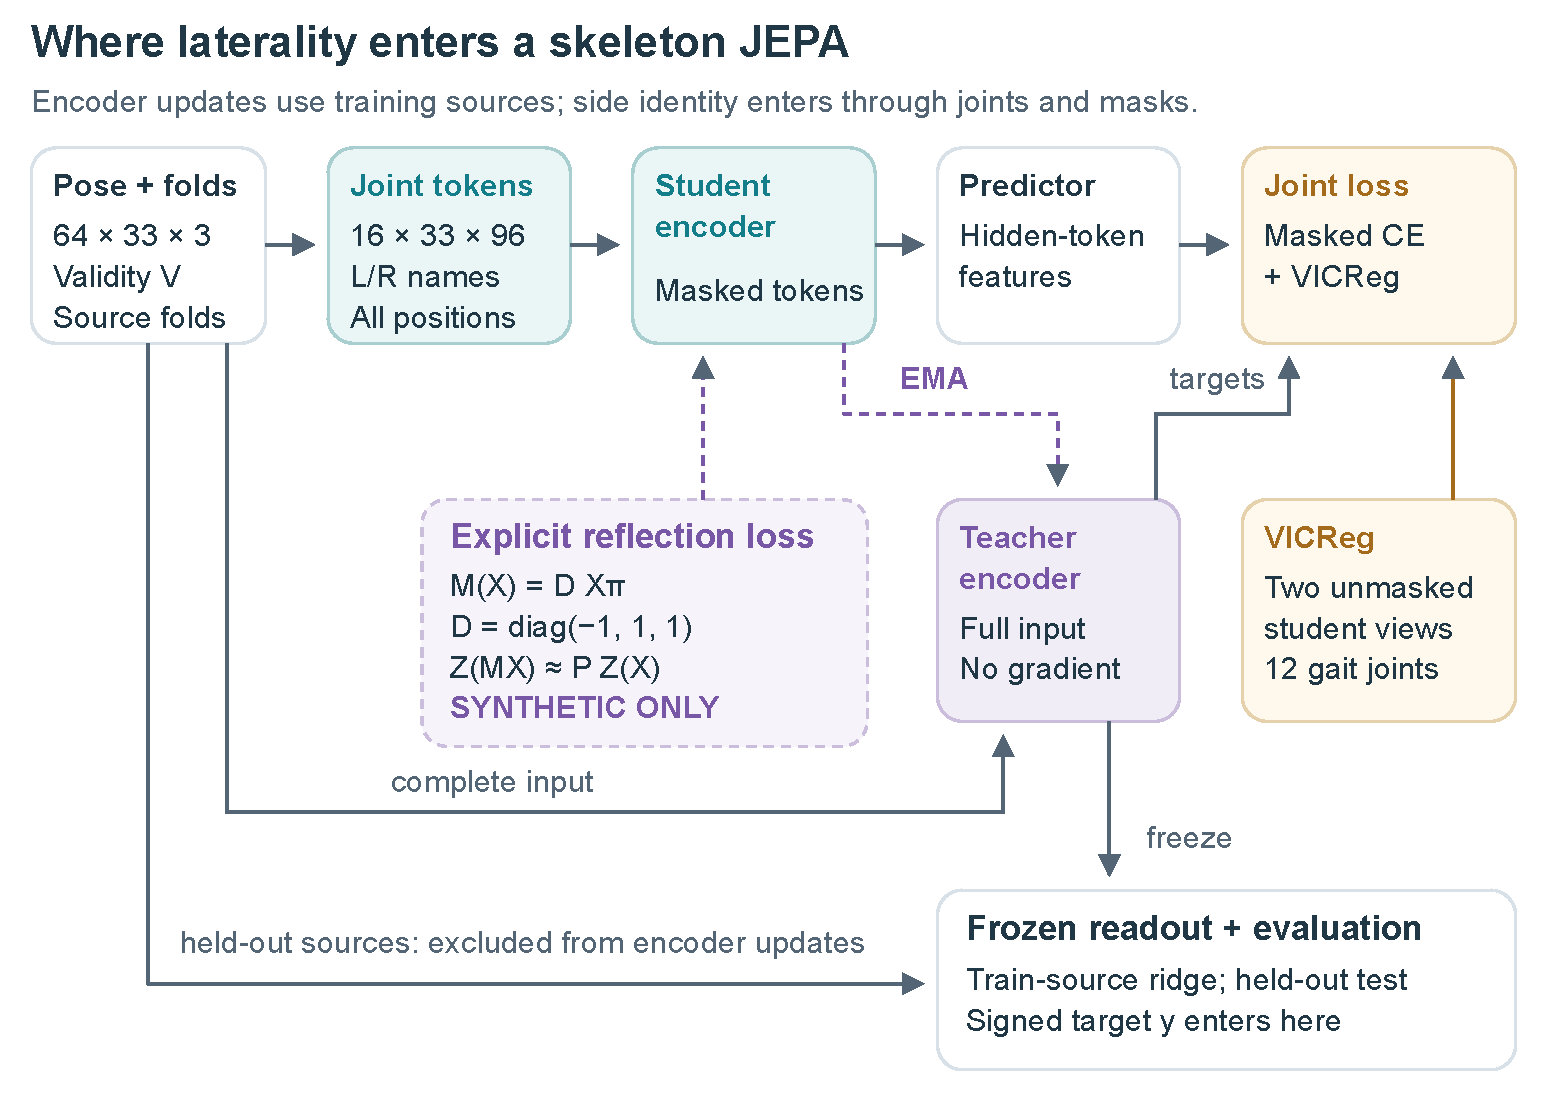
\includegraphics[width=\linewidth]{training_pipeline_compact_print.pdf}
\caption{Left-right structure enters through paired joint names, masks or pooled features based on gait joints, and an optional reflection branch. The dotted branch adds a reflection loss to the online encoder; we have tested this branch only with synthetic data. The signed movement measure is used after training, when a frozen encoder supplies features to a readout. Each clip is prepared on its own before source-fold files are written. Every training sample and transformed view keeps that source assignment.}\label{fig:training_pipeline_compact}
\end{figure}

Testing uses five outer folds. Their held-out portions contain 19, 19, 19, 18, and 18 source videos, corresponding to 189, 182, 72, 77, and 105 clips. A video's clips and augmented versions never cross folds. For every fold and random seed, a fresh encoder is trained on the other four folds, with source-balanced sampling so that videos containing many clips do not dominate.

The readout uses ridge regression, which penalizes large coefficients to limit unstable fits. Four inner folds in the reflection comparison and three in the mask and motion-readout comparisons select the penalty. Missing-value filling and scaling are fitted on each inner training split. With the selected penalty, these steps and the regression are refitted on all outer-training sources before evaluation on the held-out fold. Inner validation selects the supervised readout; its clips have already contributed without movement labels to that fold's encoder training.

The completed GAVD runs use 64 frames, 33 landmarks, 96-dimensional features, encoder/predictor depths 4/2, four attention heads, batches of 20, and 1,200 updates. Each four-frame patch is projected to a feature vector; hidden vectors are zeroed before positional information is added, retaining the full grid of positions. At hidden positions, cross-entropy matches probability distributions over teacher feature channels. The teacher receives no gradient and follows an exponential moving average of the online encoder. VICReg, weighted by 0.05 \citep{ref14}, encourages similar but nonconstant pooled features from twelve gait joints across two complete views. Its access to complete clips supplies an anatomical training signal alongside masking.

Paired mask conditions share starting weights, source draws, geometric views, and update counts, while using separate random streams for their mask policies. Each clip has its own hidden positions. Invalid targets are excluded, and losses are averaged within clips before averaging across the batch.

Reflection augmentation mirrors each training clip with probability 0.5; the motion and region mask conditions contain no reflection. We also consider an explicit reflection loss that sends the unreflected and mirrored clips through the online encoder, aligns paired joint positions, and encourages their feature channels to agree. Evidence for this loss is synthetic, and its two full-input branches add two encoder passes. Appendix B gives the details. At no point does the encoder receive the movement measure or an affected-side label.

\subsection{Testing and uncertainty}\label{testing-and-uncertainty}

For \(V\) sources and \(n_v\) clips from source \(v\), each clip has weight \(w_{vi}=1/(Vn_v)\). With \(\bar y_w=\sum w_{vi}y_{vi}\), \[
R^2_w=1-\frac{\sum_{vi}w_{vi}(y_{vi}-\hat y_{vi})^2}
{\sum_{vi}w_{vi}(y_{vi}-\bar y_w)^2}.
\] Every source video contributes equally regardless of its number of clips. Predictions from the five held-out folds are pooled within each seed to obtain one \(R^2\), and the reported score averages the five seed values. A negative score indicates greater error than a constant prediction equal to the weighted test-set mean. For deployment, a constant baseline must instead be fitted on training sources, since the new test mean would be unknown.

Grid differences are calculated from full-precision saved predictions; summary-only estimates retain the precision available in their records. Scores and interval bounds appear to three decimal places, except that a nonzero difference below 0.001 keeps one significant digit to preserve its sign.

Uncertainty is estimated by resampling whole source videos, keeping their clips and paired seed predictions together. Mask intervals compare a body- or motion-based policy with its random reference; training intervals compare an encoder with its own initialization. We did not define a smallest meaningful difference in advance, so an interval containing zero cannot establish equivalence.

For the mask and trained-versus-initial results, 2,000 resamples are drawn from the saved predictions while the fitted models and splits remain fixed. Retraining and alternative splits would add uncertainty that these intervals do not capture. The reflection comparison also used 2,000 resamples, although only its summary survives and the underlying inputs are unavailable. Seeds and mask draws reuse the same videos; they are repeated fits, not independent participants. Source holdout protects the individual comparisons from direct leakage, while repeated development on this cohort keeps the overall study exploratory.

\section{Results}\label{results}

\subsection{Preprocessing changes the measure; reflection reduces feature error}\label{preprocessing-changes-the-measure-reflection-reduces-feature-error}

Recalculating the movement measure from the prepared encoder input leaves 623 clips from 92 sources with finite values on both paths. Source-weighted sign agreement is 70.4\%, with calculation-agreement \(R^2=0.218\). Preparation therefore changes the measured target, although the contribution of individual steps remains unresolved. This comparison of calculations cannot estimate model accuracy or its upper limit.

Reflection augmentation reduces normalized feature error by \(\Delta q=-0.008\), with 95\% source interval \([-0.010,-0.007]\). Here \(q\) compares mirrored teacher features with unreflected features after exchanging joint positions and leaving feature channels unchanged. The corresponding prediction difference is \(\Delta R^2=0.004\), with interval \([-0.006,0.013]\), leaving the movement benefit uncertain. Both trained variants have greater reflection error than their initializations. These estimates survive only in the saved summary, so their uncertainty analysis could not be independently repeated.

The channel action matters: mirroring the input need not leave learned feature channels unchanged. Even perfect agreement under a chosen action can coexist with poor movement prediction. Appendix B illustrates an output formula that forces sign reversal and constant features that agree under reflection.

\subsection{Mask effects are small relative to their uncertainty}\label{mask-effects-are-small-relative-to-their-uncertainty}

For equal target counts, the saved comparison of all-landmark versus gait-joint masking gives \(\Delta R^2=0.012\), with interval \([-0.018,0.050]\). Its raw predictions are unavailable. The motion and region comparisons retain a complete prediction grid: 25 fold-and-seed jobs with three motion conditions and 25 with two region conditions, totaling 125 encoders.

The motion-mask budget is half the smallest valid gait-joint pool in each batch, rounded down, while targets are sampled across all 33 landmarks. In the saved mask-inspection draws, this averages 80.8 hidden targets, about 17\% of valid tokens over the whole body, and both motion samplers select higher-motion targets than random sampling. Connected-region inspection hides about 9.9\% of valid tokens. The fraction of hidden targets with both immediate temporal neighbors visible falls from 69.9\% to zero; the fraction with at least one visible adjacent body joint falls from 98.8\% to 51.2\%. These inspection draws describe the mask policies rather than the realized masks at every optimizer update.

\begin{table}[htbp]
\centering
\small
\begin{tabular}{@{}
  >{\raggedright\arraybackslash}p{(\linewidth - 4\tabcolsep) * \real{0.4600}}
  >{\raggedleft\arraybackslash}p{(\linewidth - 4\tabcolsep) * \real{0.2200}}
  >{\raggedright\arraybackslash}p{(\linewidth - 4\tabcolsep) * \real{0.3200}}@{}}
\toprule\noalign{}
\begin{minipage}[b]{\linewidth}\raggedright
Alternative minus its own random reference
\end{minipage} & \begin{minipage}[b]{\linewidth}\raggedleft
\(\Delta R^2\)
\end{minipage} & \begin{minipage}[b]{\linewidth}\raggedright
95\% source interval
\end{minipage} \\
\midrule\noalign{}

MAMP-style motion weighting & −0.0008 & {[}−0.020, 0.015{]} \\
Robust motion mixture & 0.0005 & {[}−0.015, 0.015{]} \\
Connected region & −0.009 & {[}−0.033, 0.018{]} \\
\bottomrule
\end{tabular}
\end{table}

All three rows cover 625 clips from 93 source videos and five seeds. Since motion and region masks use different budgets, each is paired with its own random reference. The intervals cross zero and remain compatible with small gains or losses; they support neither superiority nor equivalence. Whole-trajectory and interior-gap masks were checked for coverage but were not carried through a completed training comparison. None of the outer-test results was used to choose a winning mask.

\subsection{Trained encoders score below initialization with the expanded readout}\label{trained-encoders-score-below-initialization-with-the-expanded-readout}

Our compact summary takes the mean feature difference and sum for five left-right pairs, giving 960 regression inputs. An expanded summary adds temporal standard deviations, mean absolute changes between adjacent features, and ten values describing how much paired data is valid, for 2,890 inputs. The initial encoder's \(R^2\) rises from \(0.071\) to \(0.223\), a difference of \(0.152\). With the expanded summary, trained teachers reach \(0.101\)--\(0.114\). Every teacher scores below its initialization on \(R^2\) and above it on mean absolute error in every seed. Final online encoders also have lower \(R^2\) than their initial weights.

The initial-encoder control includes a trained pose detector, anatomical joint names, preprocessing, feature construction, and a regression fitted with movement labels. Only JEPA training is absent. The expanded summary changes several factors together: its dimension, temporal statistics, and information about missing data. Their individual contributions have not been measured, and standard deviation itself discards event order.

Paired intervals calculated from the saved predictions lie below zero for all five training arms. Under the random motion mask, for example, trained minus initial \(R^2\) is \(-0.109\), with interval \([-0.170,-0.041]\). Appendix A reports the complete set. These results locate a shortfall in the combination of this training method and readout; another readout might still recover movement information that ours misses.

For the expanded summary, 49 of 125 teacher fits (39.2\%) and 96 of 125 online-encoder fits (76.8\%) select the largest tested ridge penalty, 10,000. Extending the search through training-source validation could change the scores. A separate baseline fits ridge regression to 264 coordinate and validity summary values from prepared poses and reaches \(R^2=0.035\); more expressive coordinate models remain to be tested.

\subsection{Predictors distinguish correct clips from mismatched sources}\label{predictors-distinguish-correct-clips-from-mismatched-sources}

\begin{figure}[!tbp]
\centering
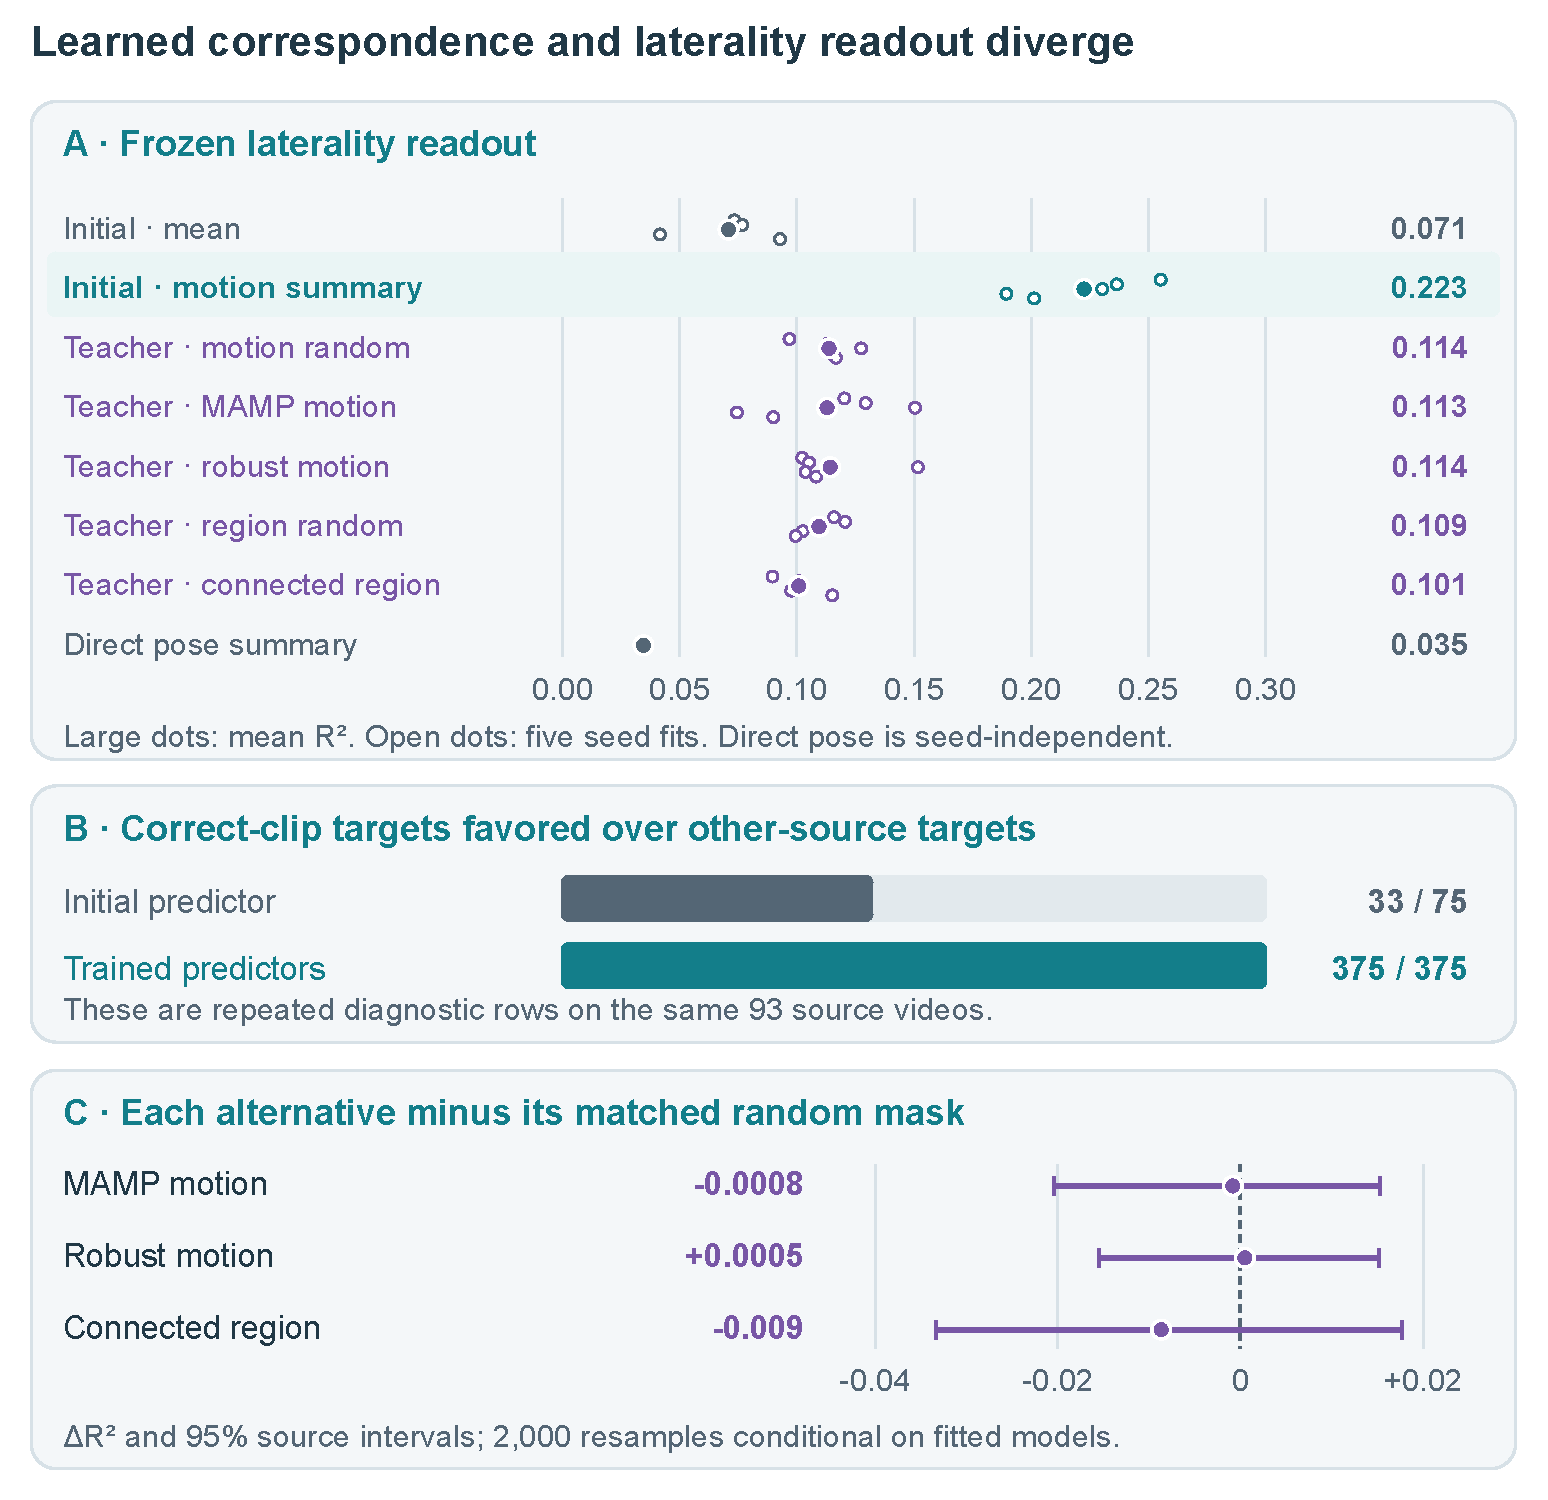
\includegraphics[width=\linewidth]{learning_results_print.pdf}
\caption{A: With the expanded summary, mean readout \(R^2\) falls from \(0.223\) at initialization to \(0.101\)--\(0.114\) after training. Points are seed scores on the same 93 videos, not confidence intervals or independent samples. B: Correct-clip feature error is lower in 375/375 trained diagnostic evaluations versus 33/75 initial evaluations. The trained evaluations cover 125 models under three masks; duplicated initial controls are counted once. C: Mask-versus-random intervals, distinct from the trained-minus-initial intervals in Appendix A. Values come from the saved prediction grid.}\label{fig:learning_results}
\end{figure}

For each diagnostic evaluation, we compare source-weighted mean squared feature error against correct-clip teacher targets and valid targets from another source, holding control clips and hidden positions fixed. Correct-clip error is lower in all 375 trained evaluations, compared with 33 of 75 initial evaluations. Each teacher target uses the full clip, so matching can draw on pose, camera view, missing-data patterns, or motion also available in the visible context. These comparisons measure clip correspondence without isolating hidden movement.

Each condition learns against its own teacher, whose feature scale and variation may differ. Consequently, raw feature losses do not provide a common scale for ranking the encoders. The movement readout supplies that shared outcome. The present diagnostics leave the cause of its training deficit unresolved.

\section{Discussion and next steps}\label{discussion-and-next-steps}

The experiments identify a deficit for this training recipe under the expanded readout. Trained features support clip correspondence, while the same regression procedure recovers more of the signed movement measure from initial features. Mask inspection confirms that the alternative policies change the available context, but their readout intervals leave gains and losses unresolved. Preparation also changes the target calculation. These observations make it premature to assign the deficit to a single cause within the encoder.

The saved encoders allow several of these possibilities to be separated without new pretraining. Missing-data support can be tested on its own, summaries can be matched in dimension, and the ridge search can be extended. Recalculating the movement measure after each preparation step would show when the disagreement enters. Any pilot used to choose among training methods needs validation videos that were excluded from both encoder training and the final regression fit.

A real-data comparison with and without the explicit reflection loss would test whether teaching the geometric relation helps movement prediction. Its readout should be compared with both the matched base model and initialization, with feature variation checked to exclude constant solutions. Compute costs need to include the extra encoder passes. The augmentation result shows why both outcomes matter: reflection error decreases, while the movement interval still crosses zero. Further confirmation requires independent sources and an evaluation plan fixed before examining their results.

Future-motion prediction would extend the work to temporal world models. Each method would receive past inputs and predict the same future coordinates, with baselines that repeat the last pose or continue recent velocity. Our present measure averages contrasts of median speed and discards event order. Testing dynamics therefore requires additional outcomes, including accuracy over forecasts rolled forward for several steps and the bilateral geometry of the predicted movement.

\section{Scope, ethics and reproducibility}\label{scope-ethics-and-reproducibility}

We chose GAVD for its clinician-annotated examples of normal and abnormal gait across clinical and less controlled recording settings \citep{ref13}. The variation in camera view and pose quality makes bilateral measurement a practical problem for Physical World AI. Walking intervals, bounding boxes, and source identifiers support traceable pose extraction and grouping of clips from a recording. Open annotations let other researchers inspect the cohort selection \citep{ref15}. Gait categories describe the selected sample and balance source splits; they do not supply encoder training labels.

Source grouping cannot rule out a person appearing in several videos. The selected sample also lacks verified affected-side labels and an independent clinical measurement of our target. Its annotations describe observed gait, while the speed contrast omits phase and loading and can cancel opposing joint differences. These limits constrain clinical interpretation and generalization beyond this cohort.

The repository carries the MIT License, copyright 2024 Rahmyyy \citep{ref16}. It permits use, modification, and redistribution of covered materials without a license fee for research or commercial purposes, with copyright and permission notices retained in copies or substantial portions. It provides no warranty and limits liability. The maintainers explicitly permit research use of the supplied annotations under these terms \citep{ref15}.

GAVD supplies video links; researchers retrieve the recordings separately under applicable platform terms, copyright, ethics, and data-protection requirements \citep{ref15}. Repository licensing alone establishes no redistribution rights for those videos or our derived pose files. Their release requires separate review. Since links may disappear, reproduction records should include the annotation version, retrieval dates, exclusions, and source splits.

We independently recalculated 200 pooled score rows and three mask intervals from 125,000 saved predictions and checked the hashes of the result tables and all 125 training histories. Checkpoint inference was not rerun; summary-only results could not be reconstructed. The {evidence records}, {recomputation script}, and {figure provenance} document the available artifacts and verification scope.
\label{physworld:main-last}
\clearpage
\label{physworld:references-start}
{\renewcommand{\bibfont}{\small}
\begin{thebibliography}{99}
\bibitem{ref01} K. K. Patterson, I. Parafianowicz, C. J. Danells, V. Closson, M. C. Verrier, W. R. Staines, S. E. Black, and W. E. McIlroy. \href{https://pubmed.ncbi.nlm.nih.gov/18226655/}{Gait asymmetry in community-ambulating stroke survivors}. \emph{Archives of Physical Medicine and Rehabilitation}, 89(2):304--310, 2008. doi:10.1016/j.apmr.2007.08.142.

\bibitem{ref02} M. D. Lewek, R. Poole, J. Johnson, O. Halawa, and X. Huang. \href{https://pubmed.ncbi.nlm.nih.gov/19945285/}{Arm swing magnitude and asymmetry during gait in the early stages of Parkinson's disease}. \emph{Gait \& Posture}, 31(2):256--260, 2010. doi:10.1016/j.gaitpost.2009.10.013.

\bibitem{ref03} S. M. Brændvik, T. Goihl, R. S. Braaten, and B. Vereijken. \href{https://pubmed.ncbi.nlm.nih.gov/32082235/}{The Effect of Increased Gait Speed on Asymmetry and Variability in Children With Cerebral Palsy}. \emph{Frontiers in Neurology}, 10:1399, 2020. doi:10.3389/fneur.2019.01399.

\bibitem{ref04} I. Vandekerckhove, M. Van den Hauwe, N. De Beukelaer, E. Stoop, M. Goudriaan, M. Delporte, G. Molenberghs, A. Van Campenhout, L. De Waele, N. Goemans, F. De Groote, and K. Desloovere. \href{https://pmc.ncbi.nlm.nih.gov/articles/PMC9201072/}{Longitudinal Alterations in Gait Features in Growing Children With Duchenne Muscular Dystrophy}. \emph{Frontiers in Human Neuroscience}, 16:861136, 2022. doi:10.3389/fnhum.2022.861136.

\bibitem{ref05} M. Abdelfattah and A. Alahi. \href{https://www.ecva.net/papers/eccv_2024/papers_ECCV/papers/04755.pdf}{S-JEPA: A Joint Embedding Predictive Architecture for Skeletal Action Recognition}. In \emph{Computer Vision -- ECCV 2024}, volume 15090 of \emph{Lecture Notes in Computer Science}, pages 367--384. Springer, 2025. doi:10.1007/978-3-031-73411-3\_21.

\bibitem{ref06} Y. Mao, J. Deng, W. Zhou, Y. Fang, W. Ouyang, and H. Li. \href{https://arxiv.org/abs/2308.07092}{Masked Motion Predictors are Strong 3D Action Representation Learners}. In \emph{Proceedings of the IEEE/CVF International Conference on Computer Vision (ICCV)}, pages 10181--10191, 2023.

\bibitem{ref07} J. Do, Y. Chen, G. Youk, and M. Kim. \href{https://arxiv.org/abs/2603.10648}{Less is More: Compact-Token Masked Feature Prediction for Skeleton Representation Learning}. arXiv preprint arXiv:2603.10648v3, 2026.

\bibitem{ref08} H. Ghaemi, E. B. Muller, and S. Bakhtiari. \href{https://proceedings.neurips.cc/paper_files/paper/2025/hash/2f63d2963526bdd9ff1b8bcc2dc9905a-Abstract-Conference.html}{seq-JEPA: Autoregressive Predictive Learning of Invariant-Equivariant World Models}. In \emph{Advances in Neural Information Processing Systems}, volume 38, pages 32943--32973, 2025. doi:10.52202/085713-1104.

\bibitem{ref09} J. Lee, C. Kim, H. Kim, K. Lee, and J. Lee. \href{https://proceedings.iclr.cc/paper_files/paper/2026/hash/3be6511c8f56d0dca4b5ed59fdf9b2f4-Abstract-Conference.html}{Soft Equivariance Regularization for Invariant Self-Supervised Learning}. In \emph{Proceedings of the International Conference on Learning Representations (ICLR)}, pages 35502--35521, 2026.

\bibitem{ref10} L. Mur-Labadia, M. Muckley, A. Bar, M. Assran, K. Sinha, M. Rabbat, Y. LeCun, N. Ballas, and A. Bardes. \href{https://arxiv.org/abs/2603.14482}{V-JEPA 2.1: Unlocking Dense Features in Video Self-Supervised Learning}. arXiv preprint arXiv:2603.14482v3, 2026.

\bibitem{ref11} H. Wei, L. Sun, and G. Zhao. \href{https://arxiv.org/abs/2608.21160}{Human-JEPA: A Human-Centric Vision Model that Perceives and Anticipates}. arXiv preprint arXiv:2608.21160v1, 2026.

\bibitem{ref12} M. J. Marin-Jimenez, I. Jimenez-Velasco, and R. Muñoz-Salinas. \href{https://github.com/AVAuco/GaitJEPA}{GaitJEPA: How Far Can We Go with JEPA on Binary Silhouettes for Gait Recognition?} \emph{IEEE International Joint Conference on Biometrics (IJCB)}, accepted paper, 2026. Author repository; accessed 10 September 2026.

\bibitem{ref13} R. Ranjan, D. Ahmedt-Aristizabal, M. Ali Armin, and J. Kim. \href{https://arxiv.org/abs/2407.04190}{Computer Vision for Clinical Gait Analysis: A Gait Abnormality Video Dataset}. \emph{IEEE Access}, 13:45321--45339, 2025. doi:10.1109/ACCESS.2025.3545787.

\bibitem{ref14} A. Bardes, J. Ponce, and Y. LeCun. \href{https://arxiv.org/abs/2105.04906}{VICReg: Variance-Invariance-Covariance Regularization for Self-Supervised Learning}. In \emph{Proceedings of the International Conference on Learning Representations (ICLR)}, 2022.

\bibitem{ref15} Rahmyyy. \href{https://github.com/Rahmyyy/GAVD/blob/a87859c881603443f200bcd640663d2c3d7a8136/README.md}{GAVD repository documentation and dataset access policy}. GitHub, n.d. README at commit a87859c; accessed 10 September 2026.

\bibitem{ref16} Rahmyyy. \href{https://github.com/Rahmyyy/GAVD/blob/a87859c881603443f200bcd640663d2c3d7a8136/LICENSE}{GAVD MIT License}. GitHub, n.d. Copyright 2024 Rahmyyy; LICENSE at commit a87859c; accessed 10 September 2026.
\end{thebibliography}
}
\clearpage
\appendix
\label{physworld:appendix-start}
\section{Trained versus initial encoders}\label{appendix-a.-trained-versus-initial-encoders}

Each final teacher encoder is compared with its own starting weights using the expanded feature summary and the same ridge-readout procedure. Every row covers 625 clips from 93 source videos and five seeds.

\begin{table}[htbp]
\centering
\small
\begin{tabular}{@{}
  >{\raggedright\arraybackslash}p{(\linewidth - 4\tabcolsep) * \real{0.4600}}
  >{\raggedleft\arraybackslash}p{(\linewidth - 4\tabcolsep) * \real{0.2200}}
  >{\raggedright\arraybackslash}p{(\linewidth - 4\tabcolsep) * \real{0.3200}}@{}}
\toprule\noalign{}
\begin{minipage}[b]{\linewidth}\raggedright
Training arm
\end{minipage} & \begin{minipage}[b]{\linewidth}\raggedleft
Learned minus initial \(R^2\)
\end{minipage} & \begin{minipage}[b]{\linewidth}\raggedright
95\% source interval
\end{minipage} \\
\midrule\noalign{}

Motion uniform & −0.109 & {[}−0.170, −0.041{]} \\
MAMP-style motion & −0.110 & {[}−0.165, −0.051{]} \\
Robust motion & −0.108 & {[}−0.171, −0.042{]} \\
Region uniform & −0.113 & {[}−0.166, −0.060{]} \\
Connected region & −0.122 & {[}−0.183, −0.055{]} \\
\bottomrule
\end{tabular}
\end{table}

The intervals come from 2,000 paired resamples of whole source videos, with each video's clips and seed predictions kept together. They condition on the fitted models and current splits, omitting uncertainty from retraining and making no adjustment for the five conditions. All intervals lie below zero for this training and expanded readout.

\section{Measurement and training details}\label{appendix-b.-measurement-and-training-details}

The target path retains original timestamps and uses transitions where both paired landmarks are observed at both ends. Pelvis centering requires both hips, and body scale is the median valid width across shoulder and hip pairs, with a unit fallback. The contrast uses \(\epsilon=10^{-8}\). The encoder path additionally fills short gaps, permits a median-pelvis fallback, and resizes to 64 positions. Their individual contributions to the measurement disagreement have not been separated. All 33 joint positions remain allocated throughout training.

The selected cohort contains 270 normal, 183 myopathic, 75 stroke, 58 cerebral-palsy, and 39 Parkinson's clips. These counts describe the sample; they identify neither the affected side nor disease prevalence.

Motion and region runs use AdamW with learning rate \(10^{-3}\), weight decay 0.05, gradient clipping at 1, and teacher EMA 0.999. Online and teacher temperatures are 0.10 and 0.06, and the target-center EMA is 0.9. The reflection-augmentation recipe schedules teacher EMA from 0.999 toward 1. Paired mask conditions match source draws, initial weights, update counts, and hidden-target counts for each clip.

The optional reflection loss compares unreflected and mirrored online-encoder features after aligning joint positions, with feature channels fixed. Squared error over positions valid in both views is divided by their combined feature energy. The denominator is held fixed during gradient calculation and bounded away from zero; clip losses are then averaged. Both branches receive gradients through two extra full-input passes. This loss has synthetic evidence only and was absent from the completed GAVD mask runs.

\begin{figure}[!tbp]
\centering
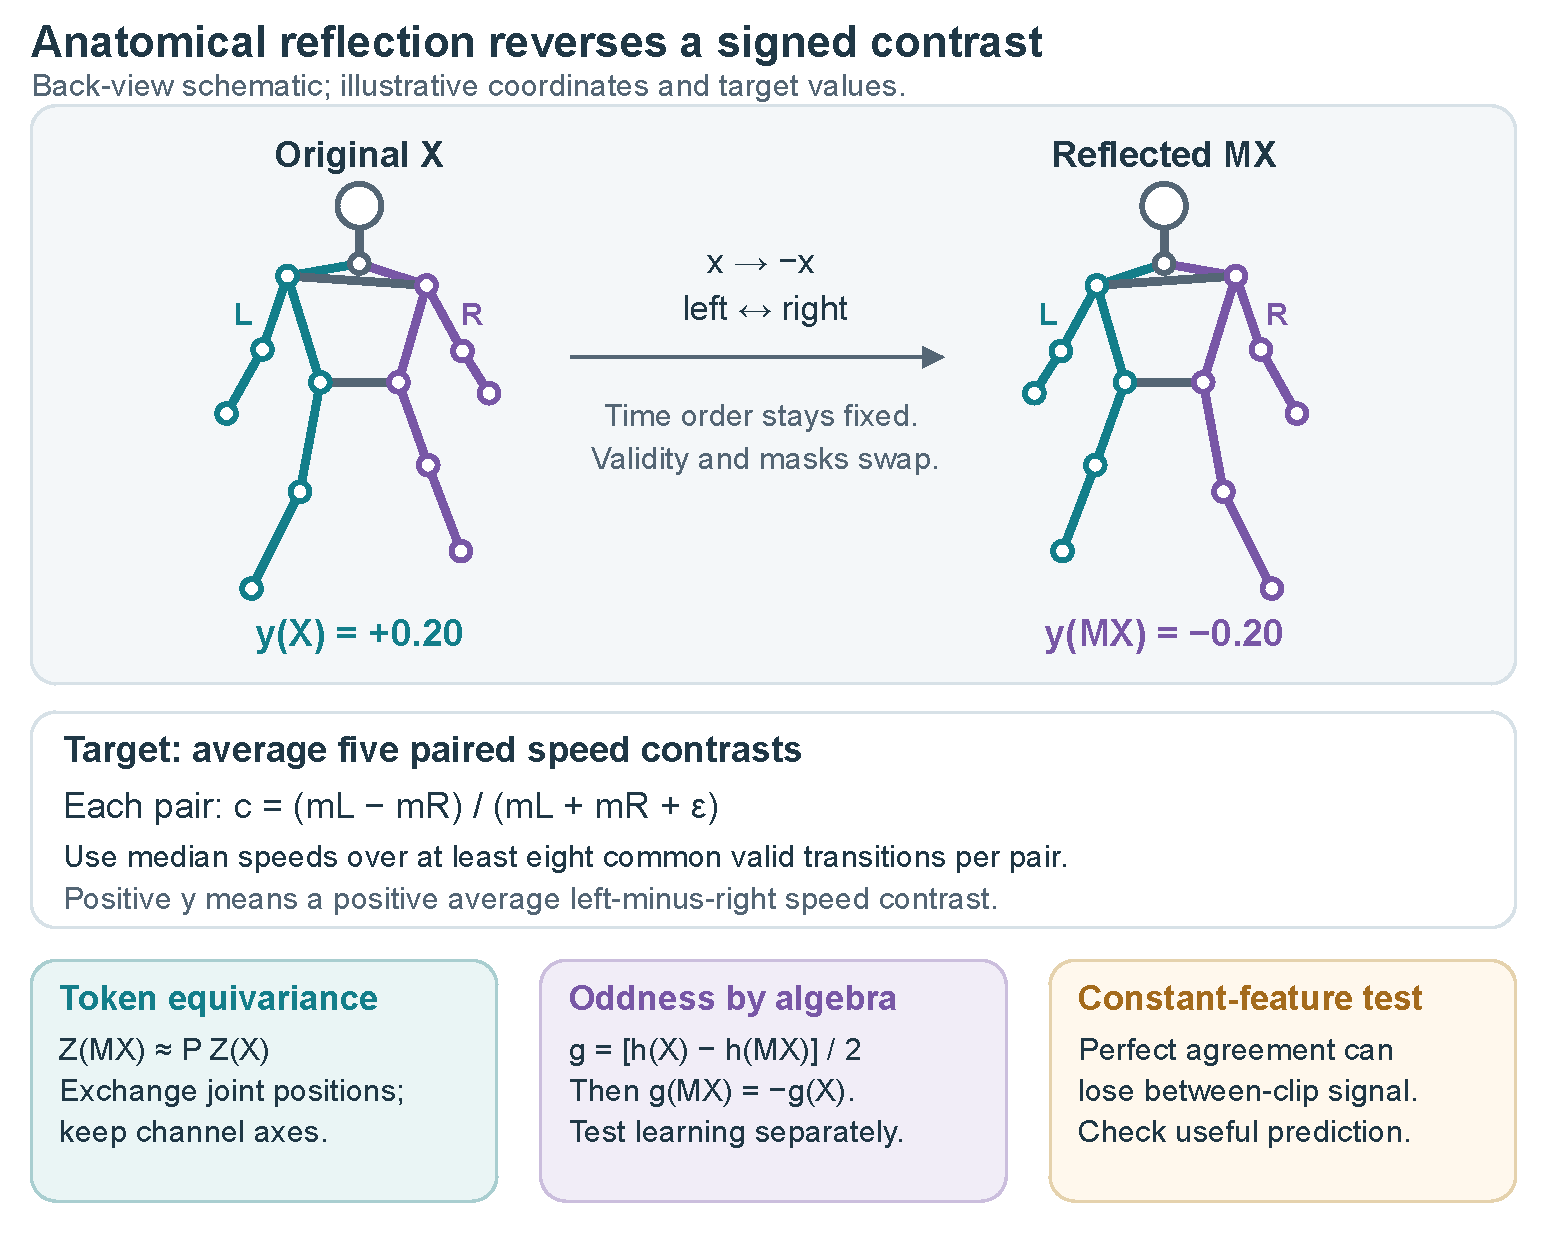
\includegraphics[width=\linewidth]{reflection_and_target_print.pdf}
\caption{Reflection swaps anatomical sides and reverses the movement measure. The lower panels illustrate two ways to satisfy symmetry without accurate movement prediction: force sign reversal in the output formula, or use constant features. Bodies and values are schematic examples.}\label{fig:reflection_and_target}
\end{figure}
\end{document}
